\documentclass{beamer}
\usepackage[utf8]{inputenc}

\usetheme{Madrid}
\usecolortheme{default}
\usepackage{amsmath,amssymb,amsfonts,amsthm}
\usepackage{txfonts}
\usepackage{tkz-euclide}
\usepackage{listings}
\usepackage{adjustbox}
\usepackage{array}
\usepackage{tabularx}
\usepackage{gvv}
\usepackage{lmodern}
\usepackage{circuitikz}
\usepackage{tikz}
\usepackage{graphicx}

\setbeamertemplate{page number in head/foot}[totalframenumber]

\usepackage{tcolorbox}
\tcbuselibrary{minted,breakable,xparse,skins}



\definecolor{bg}{gray}{0.95}
\DeclareTCBListing{mintedbox}{O{}m!O{}}{%
  breakable=true,
  listing engine=minted,
  listing only,
  minted language=#2,
  minted style=default,
  minted options={%
    linenos,
    gobble=0,
    breaklines=true,
    breakafter=,,
    fontsize=\small,
    numbersep=8pt,
    #1},
  boxsep=0pt,
  left skip=0pt,
  right skip=0pt,
  left=25pt,
  right=0pt,
  top=3pt,
  bottom=3pt,
  arc=5pt,
  leftrule=0pt,
  rightrule=0pt,
  bottomrule=2pt,
  toprule=2pt,
  colback=bg,
  colframe=orange!70,
  enhanced,
  overlay={%
    \begin{tcbclipinterior}
    \fill[orange!20!white] (frame.south west) rectangle ([xshift=20pt]frame.north west);
    \end{tcbclipinterior}},
  #3,
}
\lstset{
    language=C,
    basicstyle=\ttfamily\small,
    keywordstyle=\color{blue},
    stringstyle=\color{orange},
    commentstyle=\color{green!60!black},
    numbers=left,
    numberstyle=\tiny\color{gray},
    breaklines=true,
    showstringspaces=false,
}
%------------------------------------------------------------
%This block of code defines the information to appear in the
%Title page
\title %optional
{2.4.26}
\date{september 16,2025}


\author 
{Josyula G S Avaneesh - EE25BTECH11030}



\begin{document}



\frame{\titlepage}
\begin{frame}{Question}
Check whether (5,-2), (6,4) and (7,-2) are the vertices of an isosceles triangle.
\end{frame}



\begin{frame}{Equation}
For the points $\vec{ABC}$ to represent an isosceles triangle:\\
\textbf{Property:} The perpendicular bisector of a side passes through the opposite vertex.
\end{frame}
\begin{frame}{Theoretical Solution}

Given details:
\begin{align}
    \vec{A}=\myvec{5 \\ -2}\, \vec{B}=\myvec{6 \\ 4}\, \vec{C}=\myvec{7\\-2}
\end{align}
\end{frame}

\begin{frame}{Theoretical Solution}

\text{Midpoint of side } $\vec{AC}$: 
\begin{align}
 \vec{M} = \frac{\vec{A}+\vec{C}}{2} 
= \frac{\myvec{5\\-2}+\myvec{7\\-2}}{2} 
= \myvec{6\\-2}
\end{align}
\end{frame}


\begin{frame}{Theoretical Solution}
\text{Direction vector of side } $\vec{AC}$: 
\begin{align}
 \vec{C}-\vec{A} = \myvec{7\\-2}-\myvec{5\\-2} 
= \myvec{2\\0}
\end{align}
\text{Vector from midpoint $\vec{M}$ to } $\vec{B}$:
\begin{align}
\vec{B}-\vec{M} = \myvec{6\\4}-\myvec{6\\-2} 
= \myvec{0\\6}
\end{align}
\end{frame}
\begin{frame}{Theoretical Solution}
\begin{align}
(\vec{C}-\vec{A})^\top(\vec{B}-\vec{M}) 
= \myvec{2&0}\myvec{0\\6} = 2(0)+0(6)=0
\end{align}
\begin{align*}
 \vec{B} \text{ lies on the perpendicular bisector of side } \vec{AC}.\\
 \therefore \vec{AB} = \vec{BC} \implies \triangle ABC \text{ is isosceles.}
\end{align*}
\end{frame}


\begin{frame}[fragile]
    \frametitle{C Code (1) - Function to store the points }

    \begin{lstlisting}

#include <stdio.h>

void isosceles_triangle(double *points,double *M) {
    double coords[8] = {5,-2,  6,4,  7,-2, 6,-2};

    for (int i = 0; i < 6; i++) {
        points[i] = coords[i];
    }
    M[0]=coords[6];
    M[1]=coords[7];
}
    \end{lstlisting}
\end{frame}


\begin{frame}[fragile]
    \frametitle{Python Code - Using Shared Object}
    \begin{lstlisting}

import ctypes
import numpy as np
import matplotlib.pyplot as plt

# Load the shared object
triangle_lib = ctypes.CDLL("./triangle.so")

# Define function return type
triangle_lib.isosceles_triangle.argtypes = [np.ctypeslib.ndpointer(dtype=np.double,ndim=1,flags="C"),np.ctypeslib.ndpointer(dtype=np.double, ndim=1, flags="C")]


\end{lstlisting}
\end{frame}

\begin{frame}[fragile]
    \frametitle{Python Code - Using Shared Object}
    \begin{lstlisting}
# Create numpy array to hold 6 values (x,y for 3 points)
points = np.zeros(6, dtype=np.double)
M = np.zeros(2, dtype=np.double)

# Call C function to fill points
triangle_lib.isosceles_triangle(points,M)

# Reshape into (3,2)
points = points.reshape((3,2))

# Close the triangle (repeat first point)
points = np.vstack([points, points[0]])

\end{lstlisting}
\end{frame}
\begin{frame}[fragile]
    \frametitle{Python Code - Using Shared Object}
    \begin{lstlisting}
#text
plt.text(points[0,0]+0.2, points[0,1]+0.2, "A(5,-2)", fontsize=12, ha='right')
plt.text(points[1,0], points[1,1], "B(6,4)", fontsize=12, ha='right')
plt.text(points[2,0]+0.2, points[2,1]+0.2, "C(7,-2)", fontsize=12, ha='left')
plt.text(M[0]+0.2, M[1]+0.2, "M(6,-2)", fontsize=12, ha='center')





\end{lstlisting}
\end{frame}

\begin{frame}[fragile]
     \frametitle{Python Code - Using Shared Object}
     \begin{lstlisting}
         # Plot isosceles triangle
plt.plot(points[:,0], points[:,1], "bo-")
plt.plot([M[0],points[1,0]],[M[1],points[1,1]],"go-")
plt.xlim([2,9])
plt.ylim([-4,6])
plt.title("isosceles triangle from C library")
plt.xlabel("X-axis")
plt.ylabel("Y-axis")
plt.gca().set_aspect("equal")
plt.grid(True)
plt.savefig('figs/triangle.png')
plt.show()
     \end{lstlisting}
     \end{frame}


\begin{frame}{Plot-Using Both C and Python}
    \centering
    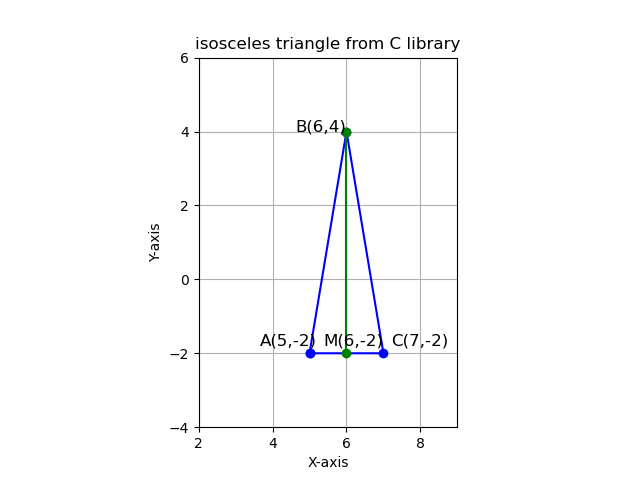
\includegraphics[width=\columnwidth, height=0.8\textheight, keepaspectratio]{figs/triangle.png}     
\end{frame}

\begin{frame}[fragile]
    \frametitle{Python Code}
    \begin{lstlisting}
import numpy as np
import matplotlib.pyplot as plt

# Define the vertices of the triangle
points = np.array([
    [5, -2],   # A
    [6, 4],   # B
    [7, -2], # C

])
M=np.array([6,-2])





\end{lstlisting}
\end{frame}

\begin{frame}[fragile]
    \frametitle{Python Code }
    \begin{lstlisting}
# Close the triangle (repeat first point)
points = np.vstack([points, points[0]])

#scatter
plt.text(points[0,0]+0.2, points[0,1]+0.2, "A(5,-2)", fontsize=12, ha='right')
plt.text(points[1,0], points[1,1], "B(6,4)", fontsize=12, ha='right')
plt.text(points[2,0]+0.2, points[2,1]+0.2, "C(7,-2)", fontsize=12, ha='left')
plt.text(M[0]+0.2, M[1]+0.2, "M(6,-2)", fontsize=12, ha='center')


\end{lstlisting}
\end{frame}

\begin{frame}[fragile]
    \frametitle{Python Code }
    \begin{lstlisting}
#Plot
plt.plot([M[0],points[1,0]],[M[1],points[1,1]],"go-",linewidth=2)
plt.plot(points[:,0], points[:,1], "bo-", linewidth=2)
plt.xlim([2,9])
plt.ylim([-4,6])
plt.title("isosceles triangle")
plt.xlabel("X-axis")
plt.ylabel("Y-axis")
plt.gca().set_aspect("equal")
plt.grid(True)
plt.savefig('figs/triangle2.png')
plt.show()

\end{lstlisting}
\end{frame}


\begin{frame}{Plot-Using only Python}
    \centering
    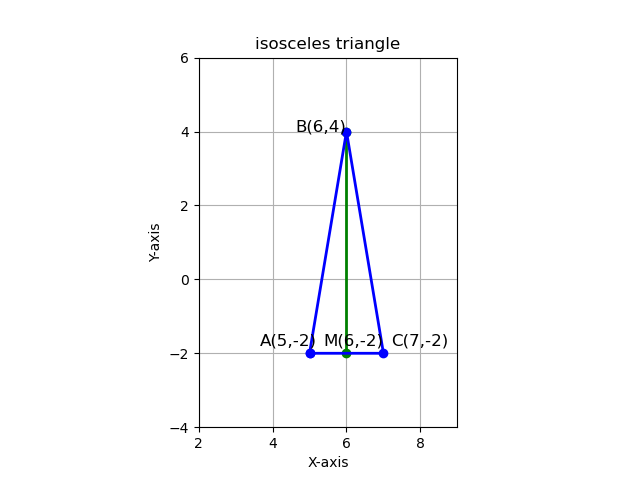
\includegraphics[width=\columnwidth, height=0.8\textheight, keepaspectratio]{figs/triangle2.png}     
\end{frame}


\end{document}